\section{WebApp}
\label{sec:webapp}
Una applicazione web è una applicazione client/server per un ambiente stateless, cioè senza memoria, che utilizza le tecnologie internet. Con il termine Webapp si descrive un'applicazione accessibile via web per mezzo di una network, come ad esempio una Intranet o attraverso la rete Internet. Pertanto, saper programmare per il web significa conoscere i diversi meccanismi e strumenti per conservare o passare i dati, detti parametri, tra le diverse pagine dell'applicazione web. In pratica una Web-application, è un programma che non necessita di essere installato nel computer in quanto esso si rende disponibile su un server in rete e può essere fatto funzionare attraverso un normale Web browser (es. Google Chrome, Mozilla Firefox, Opera, ecc.) in posizione di client. Il client, dopo aver instaurato una connessione con il server, invia la richiesta per un servizio; il server dopo aver elaborato i dati necessari rende disponibile al client il servizio richiesto. A differenza dei siti web statici (HTML), l'applicazione web viene realizzata con una o più tecnologie (Javascript, Ajax, Servlet, Database ecc.) che permettono la creazione di un sito dinamico, cioè di un sito nel quale il contenuto delle pagine varia durante l'interazione.
\\Le applicazioni Web si pongono come valida alternativa alle tradizionali applicazioni Client/Server per vari motivi:
\begin{itemize}
\item \textit{Facilità di distribuzione e aggiornamento}: un'applicazione Web risiede interamente sul server, per cui la sua pubblicazione coincide con la distribuzione e l'aggiornamento ed è automaticamente disponibile a tutti gli utenti.
\item \textit{Accesso multi-piattaforma}: l'accesso all'applicazione è indipendente dall'hardware e dal sistema operativo utilizzato dagli utenti;
\item \textit{Riduzione del costo di gestione}: l'uso di Internet come infrastruttura per un'applicazione Web riduce notevolmente sia i costi di connettività che i costi di gestione dei client;
\item \textit{Scalabilità}: un'applicazione Web ben progettata può crescere insieme alle esigenze dell'azienda senza particolari problemi;
\end{itemize}
Per poter mostrare l'elaborazione di Spark nel sistema distribuito, si è preferito utilizzare una webapp per i motivi sopra citati. Questa applicazione web fa uso di tecnologie di ultima generazione quali NodeJs ed HTML5. Questo la rende fruibile a tutti gli utenti provvisti di Pc, Tablet o Smartphone con un browser installato. Nel seguente capito dunque vengono messi in luce i principali componenti che compongono la webapp, mostrando i punti forti di ogni tecnologia.
\begin{figure}[H]
	\centering
	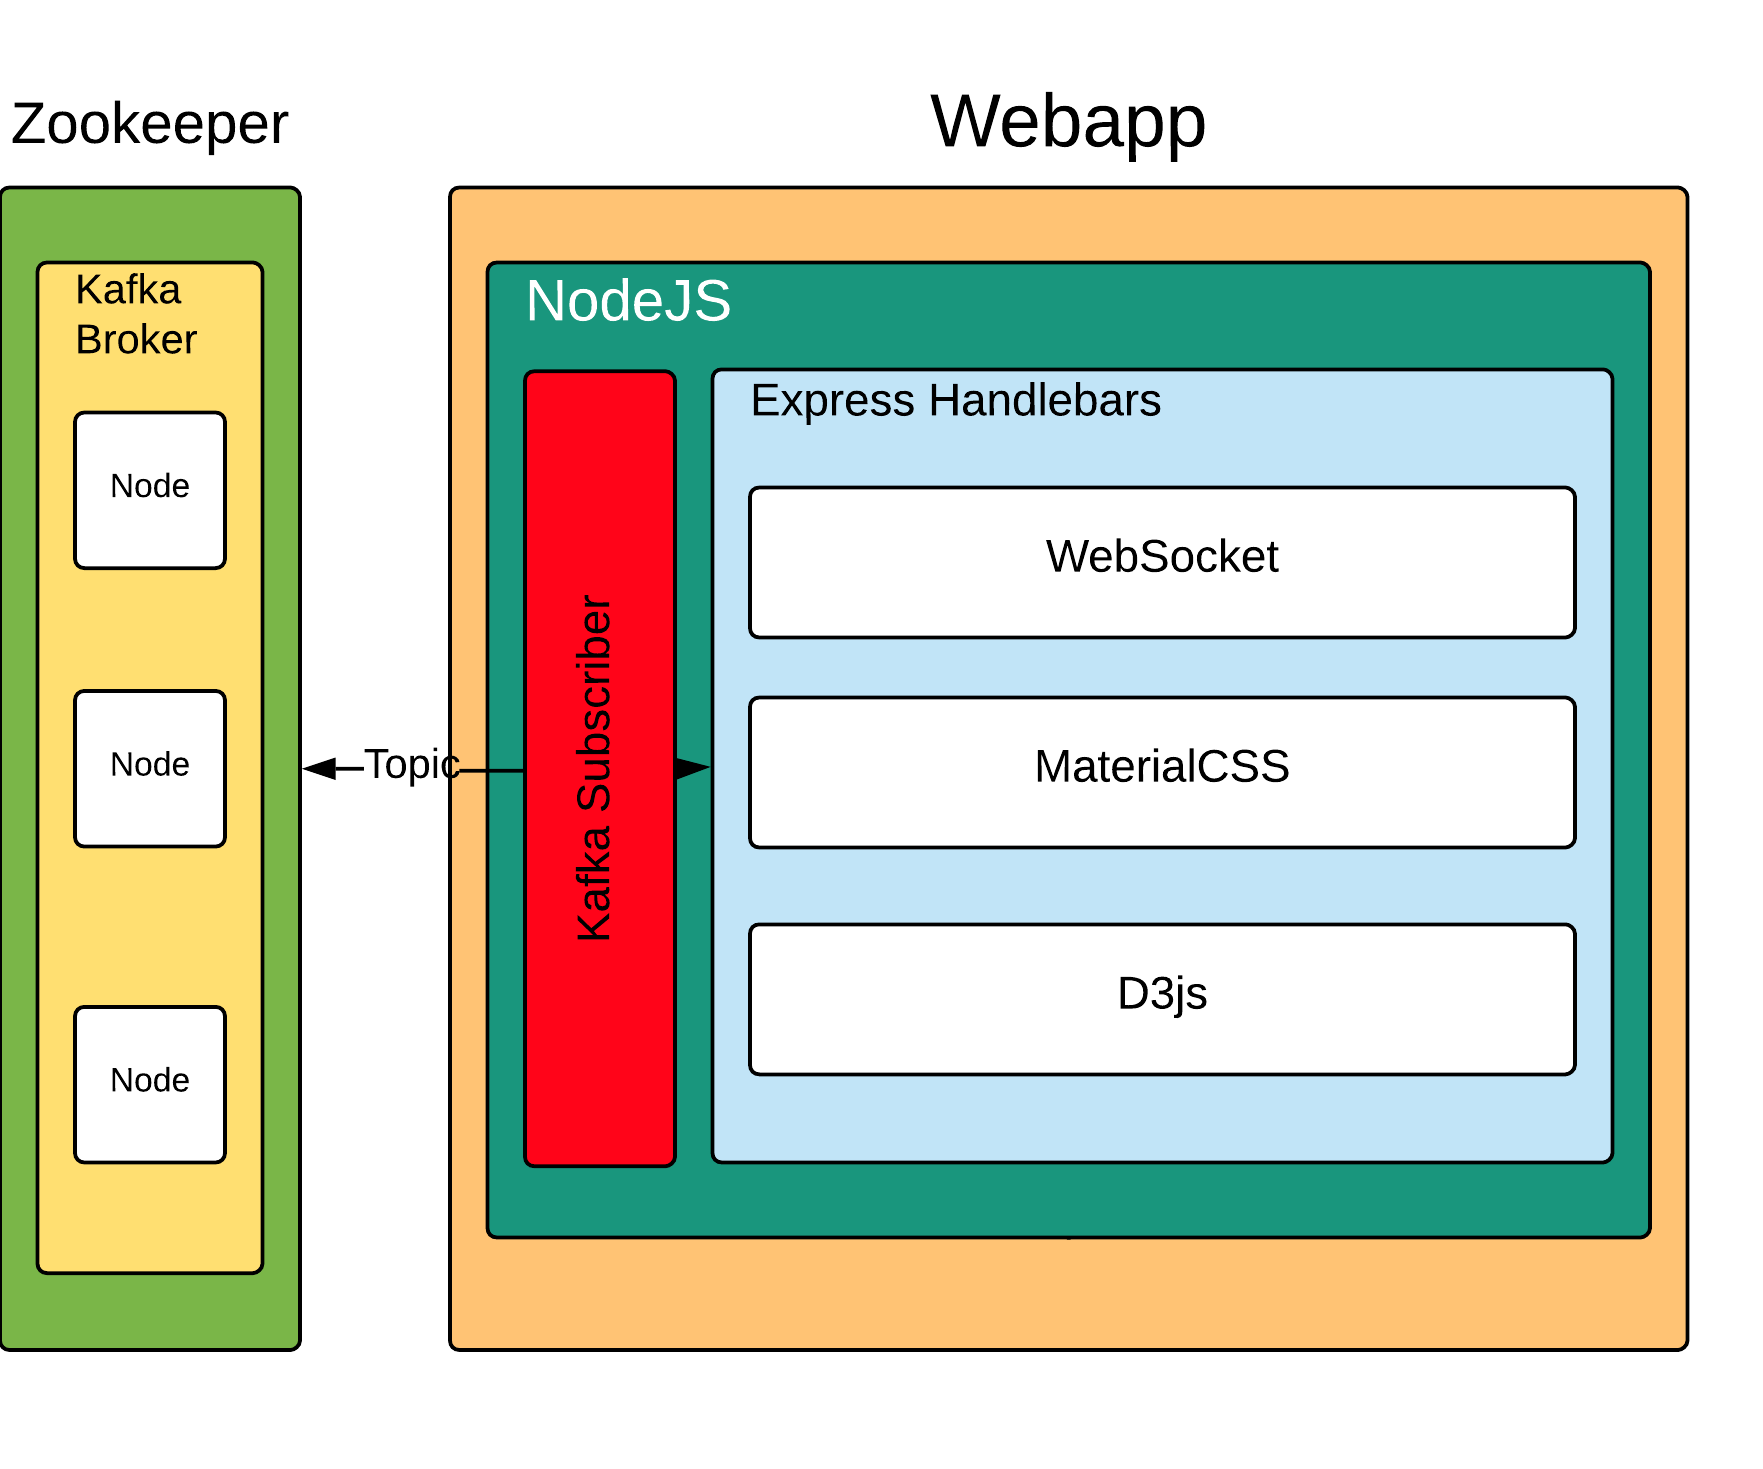
\includegraphics[width=\textwidth]{images/webApp.png}
	\caption{Architettura in dettaglio della webapp.}
	\label{fig:webAppArchitetture}
\end{figure}